\section{Evaluation}

\subsection{Lucene Evaluation}

We begin by quantifying the performance impact of static and dynamic DRAM partitioning under varying budgets. 
For both the M1 and M2 workloads, we collect metrics including total execution time, 
young GC time, mixed/full GC time. These metrics highlight how each configuration 
responds to increasing memory pressure.

Figures~\ref{fig:m1-exec} and~\ref{fig:m2-exec} summarize the normalized execution time breakdown for both workloads.
Each DRAM setting is shown as a pair of bars: the left bar corresponds to the static TeraHeap (TH) configuration, 
and the right to the dynamic FlexHeap (FH). All bars are normalized to the TeraHeap execution time. 

Each bar is split into three regions: 
light gray indicates non-GC execution time, 
blue represents young GC time, 
and orange captures mixed or full GC time.


\begin{figure}[htbp]
  \centering
  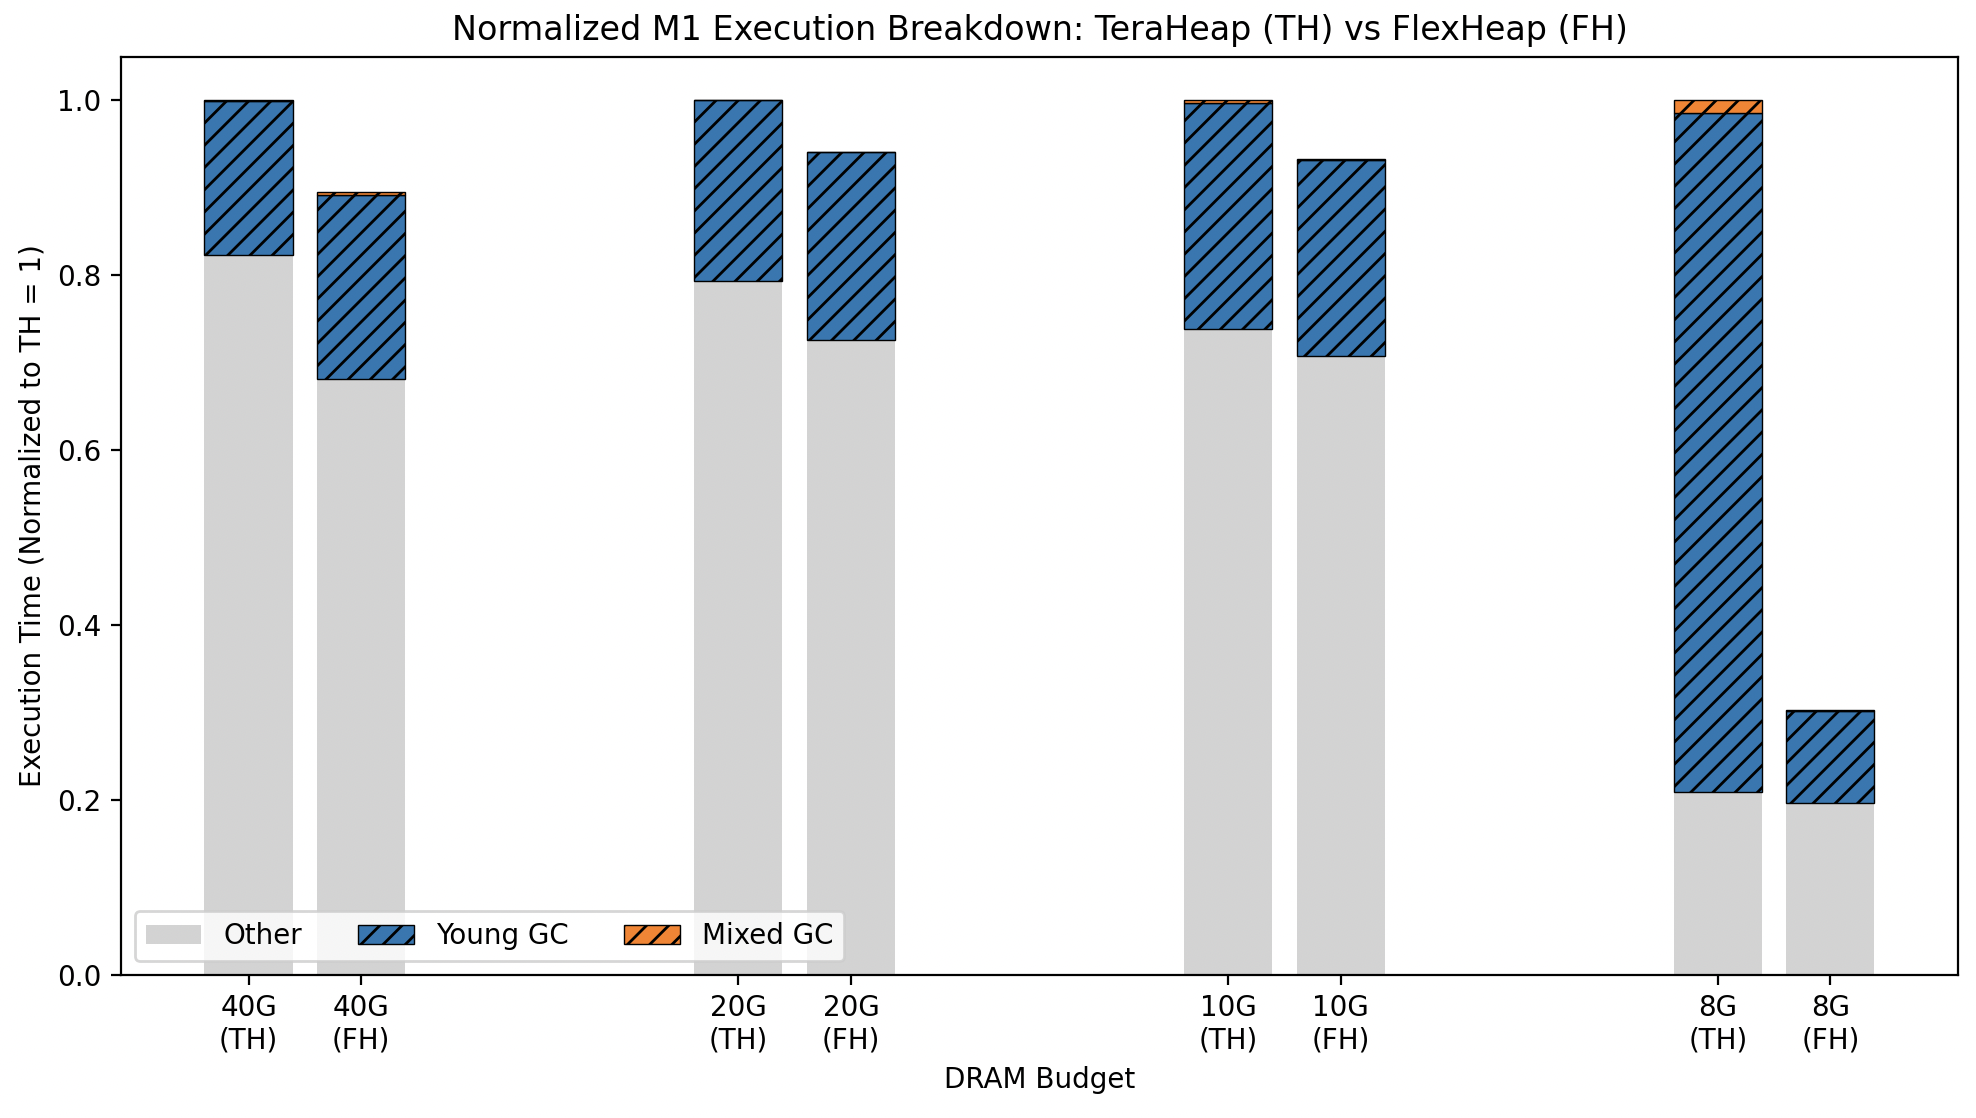
\includegraphics[width=0.95\linewidth]{fig/M1_exec.png}
  \caption{Normalized execution time breakdown for M1 workload across different DRAM budgets using TeraHeap (TH) and FlexHeap (FH).}
  \label{fig:m1-exec}
\end{figure}

\begin{figure}[htbp]
  \centering
  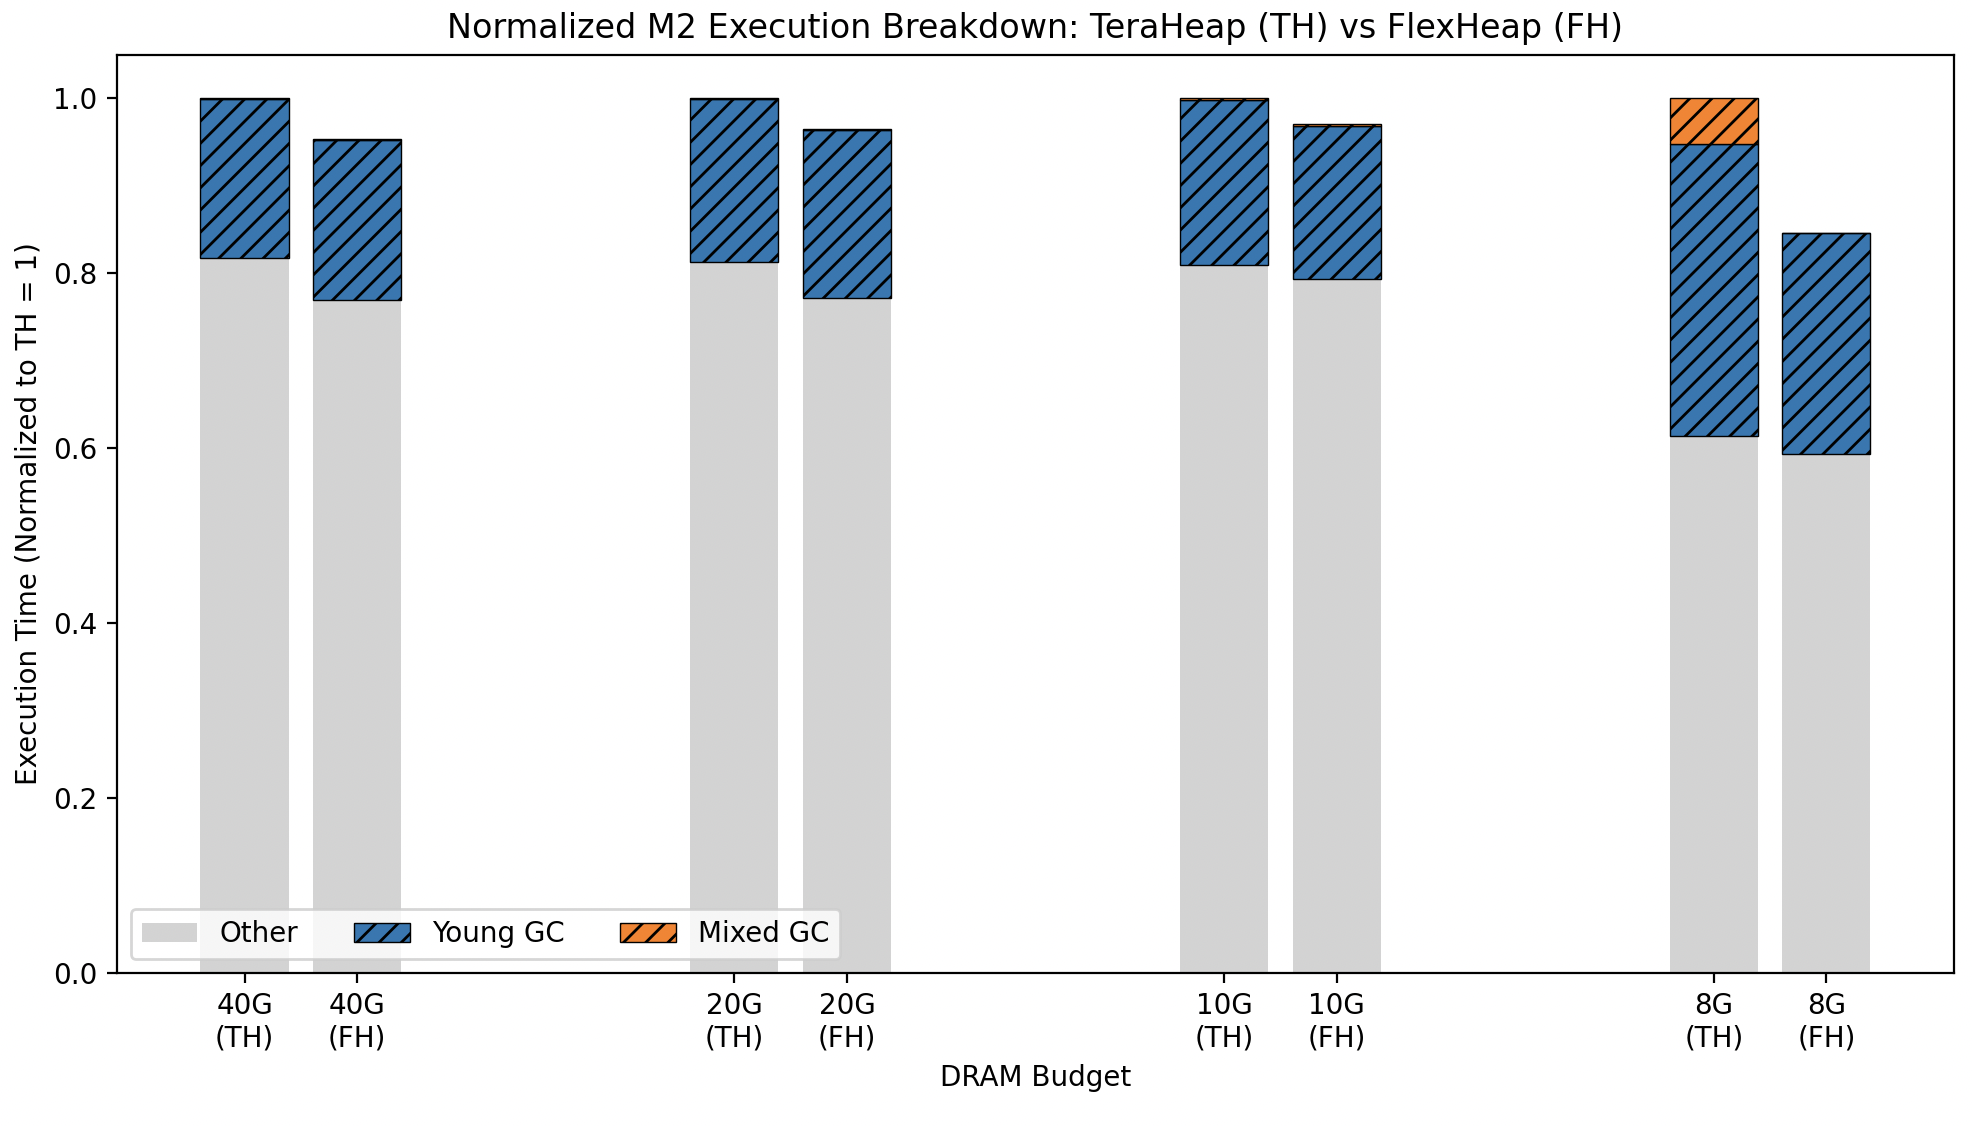
\includegraphics[width=0.95\linewidth]{fig/M2_exec.png}
  \caption{Normalized execution time breakdown for M2 workload across different DRAM budgets using TeraHeap (TH) and FlexHeap (FH).}
  \label{fig:m2-exec}
\end{figure}

We also measure total read and write traffic on the device hosting the H2 file during each benchmark run. 
These values reflect the pressure placed on the OS page cache and illustrate how dynamic heap resizing 
can mitigate unnecessary page faults and evictions.

\begin{table}[h]
\centering
\caption{Read and Write Traffic for M1 workload (in GB)}
\label{tab:m1-traffic}
\begin{tabular}{|c|cc|cc|}
\hline
\textbf{DRAM} & \multicolumn{2}{c|}{\textbf{Read Traffic (GB)}} & \multicolumn{2}{c|}{\textbf{Write Traffic (GB)}} \\
\textbf{Budget} & TH & FH & TH & FH \\
\hline
40G & 0,938 & 2,039 & 104,075  & 109,4 \\
20G & 44,823 & 2,854 & 107,866 & 107,231 \\
10G & 287,303 & 25,653 & 108,43 & 109,018 \\
8G  & 249,536 & 85,598 & 115,64 & 107,125 \\
\hline
\end{tabular}
\end{table}

\begin{table}[h]
\centering
\caption{Read and Write Traffic for M2 workload (in GB)}
\label{tab:m2-traffic}
\begin{tabular}{|c|cc|cc|}
\hline
\textbf{DRAM} & \multicolumn{2}{c|}{\textbf{Read Traffic (GB)}} & \multicolumn{2}{c|}{\textbf{Write Traffic (GB)}} \\
\textbf{Budget} & TH & FH & TH & FH \\
\hline
40G & 0,679 & 0,292 & 94,396  & 100,393 \\
20G & 11,402 & 0,895 & 97,591 & 97,912 \\
10G & 109,527 & 12,18 & 99,238 & 99,239 \\
8G  & 50,936 & 516,566 & 98,553 & 98,274 \\
\hline
\end{tabular}
\end{table}

\vspace{1em}

